% Orbit-Evidence -- ADVISOR REVIEW deck. 23 main frames + 12 appendix. VISUAL-FIRST. 20-30 min with interruption.
%
% THIS IS NOT THE WORKSHOP TALK. The reviewer-proof workshop deck lives at
% talk/orbit_evidence_talk.tex (tag talk/orbit-evidence-reviewer-proof-2026-08) and is untouched.
% This deck exists to let an advisor CRITIQUE the research: it explains the method rather than
% summarising it, and it carries a submission-positioning slide that must never appear publicly.
%
% NO OVERLAYS. The advisor may receive only a static PDF, so every frame is final-state: logical
% slide count equals physical page count. A 35-page PDF that is really 23 slides is worse than no
% animation at all.
%
% SOURCE OF TRUTH. Every number comes from numbers.tex, generated by gen_numbers.py from three
% frozen artifacts. Do not type a number into a slide.
%
% SCOPE. This deck presents no Doppler-residual, LR-FHSS, RF, or conducted-IQ result as a
% contribution. The stopped research line appears once, in appendix A10, explicitly labelled as
% historical motivation only.
\documentclass[aspectratio=169,11pt]{beamer}

\usetheme[progressbar=frametitle, numbering=fraction, block=fill]{metropolis}
\usefonttheme{professionalfonts}

\usepackage{appendixnumberbeamer}
\usepackage{amsmath,amssymb}
\usepackage{tikz}
\usetikzlibrary{arrows.meta,positioning,fit,backgrounds,calc}
\usepackage{booktabs}
\usepackage{xcolor}

\newcommand{\rulename}[1]{\textsf{#1}}
% GENERATED by talk/advisor_review/gen_numbers.py -- do not edit.
% Sources: evaluation/results/final_summary.json,
%          evaluation/real_data/l47_alongtrack.json,
%          evaluation/results/l47_power_curve.json
% Retyping any of these into a slide removes the only guard against a stale figure.
\newcommand{\Nrules}{19}
\newcommand{\Nfaults}{17}
\newcommand{\Ncontract}{17}
\newcommand{\Nred}{16}
\newcommand{\Nnored}{3}
\newcommand{\Nchrono}{2}
\newcommand{\Nenvs}{3}
\newcommand{\Nconds}{18}
\newcommand{\Nstatechannels}{6}
\newcommand{\Ncleanhalts}{14}
\newcommand{\Ncleanpaths}{450}
\newcommand{\Nrate}{0.031}
\newcommand{\Nwlo}{0.018}
\newcommand{\Nwhi}{0.052}
\newcommand{\Nalpha}{0.05}
\newcommand{\Nseeds}{40}
\newcommand{\Nrholo}{0.2}
\newcommand{\Nrhohi}{0.8}
\newcommand{\Npowerlo}{0.25}
\newcommand{\Nhaltslo}{10}
\newcommand{\Nhaltshi}{40}
\newcommand{\NpermB}{400}
\newcommand{\Ncalgroups}{8}
\newcommand{\Ncalunits}{3}
\newcommand{\Nmingroups}{4}
\newcommand{\Nminunits}{8}
\newcommand{\Nbootdraws}{2000}
\newcommand{\Nassignthree}{15}
\newcommand{\Nminpthree}{0.0667}
\newcommand{\Nassignfour}{105}
\newcommand{\Nminpfour}{0.0095}
\newcommand{\Npasses}{331}
\newcommand{\Nelsets}{109}
\newcommand{\Nobjects}{11}
\newcommand{\Natused}{272}
\newcommand{\Natelsets}{90}
\newcommand{\Natdropped}{59}
\newcommand{\Naticc}{0.501}
\newcommand{\Natp}{0.0025}
\newcommand{\Natlo}{0.376}
\newcommand{\Natupper}{0.638}
\newcommand{\Naticcobj}{0.241}
\newcommand{\Naticcelset}{0.284}
\newcommand{\Nelevicc}{0.000}
\newcommand{\Nelevp}{1.000}
\newcommand{\Nelevunits}{305}
\newcommand{\Nelevgroups}{101}
\newcommand{\Natmedian}{0.226}
\newcommand{\Nlagmedian}{6.36}
\newcommand{\Nlagobjects}{11}
\newcommand{\Nextrules}{19}
\newcommand{\Nextpass}{5}
\newcommand{\Nexthalt}{3}
\newcommand{\Nextindet}{1}
\newcommand{\Nextna}{5}
\newcommand{\Nextnobs}{5}
\newcommand{\Nextadjudicated}{9}
\newcommand{\Nextnoverdict}{10}
\newcommand{\Nconsseeds}{5}
\newcommand{\Nconschanged}{5}
\newcommand{\Nconsoverlap}{100.0}
\newcommand{\Nconsoverlapcorr}{0}
\newcommand{\Nwindowspan}{260}
\newcommand{\Nboundarydropped}{259}
\newcommand{\Nconsminp}{0.0625}
\newcommand{\Nclaimsites}{64}
\newcommand{\Nloc}{833}


\definecolor{oeaccent}{HTML}{1B4965}
\definecolor{oelight}{HTML}{E8F0F6}
\definecolor{oegrey}{HTML}{5A6B78}
\definecolor{oewarn}{HTML}{9C4221}   % restrained red: invalid / prohibited paths only
\setbeamercolor{frametitle}{bg=oeaccent}
\setbeamercolor{progress bar}{fg=oewarn}
\setbeamercolor{alerted text}{fg=oewarn}

% One message per slide.
\newcommand{\msg}[1]{%
  \vfill\vspace{0.2em}%
  \begin{center}\begin{minipage}{0.94\textwidth}\centering
  \small\itshape\color{black!70}#1
  \end{minipage}\end{center}}
\newcommand{\msgflush}[1]{%
  \vspace{0.4em}%
  \begin{center}\begin{minipage}{0.94\textwidth}\centering
  \small\itshape\color{black!70}#1
  \end{minipage}\end{center}}

% A boxed "do not conclude" note. Red is reserved for exactly this.
% \par first: without it this ran on from the preceding sentence, so the boundary statement
% read as a continuation of the result rather than a limit on it.
% Short attribution for a borrowed primitive. Each resolves to a paper/refs.bib entry and is
% listed in full on A12. The deck previously named ICC(1), permutation inference, metamorphic
% testing and hermetic closure with no attribution at all, which is an integrity gap in a deck
% whose whole argument is that it invented none of its primitives.
\newcommand{\srcref}[1]{{\scriptsize\color{oegrey}[#1]}}

\newcommand{\notclaim}[1]{%
  \par\vspace{0.45em}%
  {\small\color{oewarn}\textbf{Not claimed:} #1\par}}

\tikzset{
  stage/.style={draw=oeaccent, line width=0.6pt, fill=oelight, align=center,
                text width=17mm, minimum height=9mm, inner sep=1mm, font=\scriptsize},
  layer/.style={draw=oegrey, line width=0.6pt, fill=black!3, align=left,
                text width=25mm, minimum height=12mm, inner sep=1.2mm, font=\scriptsize},
  panel/.style={draw=oeaccent, line width=0.7pt, fill=oelight, align=center,
                inner sep=1.5mm, font=\scriptsize},
  bad/.style={draw=oewarn, line width=0.7pt, fill=oewarn!8, align=center,
              inner sep=1.5mm, font=\scriptsize},
  flow/.style={-{Latex[length=1.4mm]}, line width=0.6pt, oegrey},
  rel/.style={{Latex[length=1.4mm]}-{Latex[length=1.4mm]}, line width=1.0pt, oeaccent},
  % ---- visual-first redesign styles. The advisor reads figures, not paragraphs, so the deck
  % needs a small vocabulary of shapes it can reuse: a titled card, a tree node, a bar, a
  % verdict chip. Defined once here so every slide looks like the same deck.
  card/.style={draw=oeaccent, line width=0.7pt, fill=oelight, rounded corners=1pt,
               align=center, text width=32mm, minimum height=15mm, inner sep=1.6mm,
               font=\scriptsize},
  cardbad/.style={card, draw=oewarn, fill=oewarn!7},
  cardgood/.style={card, draw=oeaccent!70, fill=oeaccent!7},
  hdr/.style={font=\scriptsize\bfseries, color=oeaccent},
  tnode/.style={draw=oeaccent, line width=0.6pt, fill=oelight, rounded corners=1pt,
                align=center, inner sep=1mm, font=\scriptsize, minimum height=5.5mm},
  tleaf/.style={draw=oegrey, line width=0.5pt, fill=black!3, align=center, inner sep=0.8mm,
                font=\tiny, minimum height=4.5mm, text width=11mm},
  tree/.style={-{Latex[length=1.1mm]}, line width=0.5pt, oegrey},
  bar/.style={fill=oeaccent, draw=none},
  barlo/.style={fill=oegrey!45, draw=none},
  chip/.style={draw=oegrey, line width=0.5pt, align=center, inner sep=0.8mm,
               font=\scriptsize, minimum width=9mm, minimum height=7mm},
  big/.style={font=\Large\bfseries, color=oeaccent},
}

% \tick / \cross are used as inline MARKS inside node text, so they must be commands, not
% tikz styles -- defining them in \tikzset made \tick{...} an undefined control sequence.
\newcommand{\tick}[1]{{\bfseries\color{oeaccent}#1}}
\newcommand{\cross}[1]{{\bfseries\color{oewarn}#1}}

% One large takeaway line, for slides whose whole point is a single sentence under a figure.
\newcommand{\ruletag}[1]{{\par\vspace{-1.0em}\hfill{\tiny\color{oegrey}#1}\par\vspace{0.1em}}}
\newcommand{\punch}[1]{%
  \vfill
  \begin{center}\begin{minipage}{0.94\textwidth}\centering
  \normalsize\bfseries\color{oeaccent}#1
  \end{minipage}\end{center}}

\title{Orbit-Evidence}
\subtitle{Relational Validity Checks for Learning-Assisted\\Satellite Communication Experiments}
\date{Advisor review --- pre-submission}
\author{Advisor review deck (not for public presentation)}

\begin{document}

% ================================================================= ACT I -- title
% 1 ---------------------------------------------------------------- title + thesis
{\setbeamercolor{background canvas}{bg=oeaccent}
 \setbeamercolor{normal text}{fg=white}
 \begin{frame}[plain]
 \usebeamercolor[fg]{normal text}
 \vfill
 {\Large\textbf{Orbit-Evidence}}\\[0.4em]
 {\normalsize Relational Validity Checks for Learning-Assisted\\Satellite Communication
  Experiments}\\[1.4em]
 \textcolor{white!45}{\rule{0.28\textwidth}{0.6pt}}\\[0.9em]
 {\normalsize Some deployment-validity failures cannot be seen\\
  inside one realised dataset.}
 \vfill
 {\scriptsize\color{white!60}Advisor review --- pre-submission. Not the public workshop talk.}
 \end{frame}}

% ================================================================= ACT I -- the problem, in pictures
% 2 ---------------------------------------------------------------- the pipeline being validated
% 2 ---------------------------------------------------------------- what the experiment does
% The advisor is not a satellite specialist, so this slide teaches the actual system rather than a
% generic pipeline: what goes in, where learning sits, and what the decision is.
\begin{frame}{The kind of experiment this work audits}
  \centering
  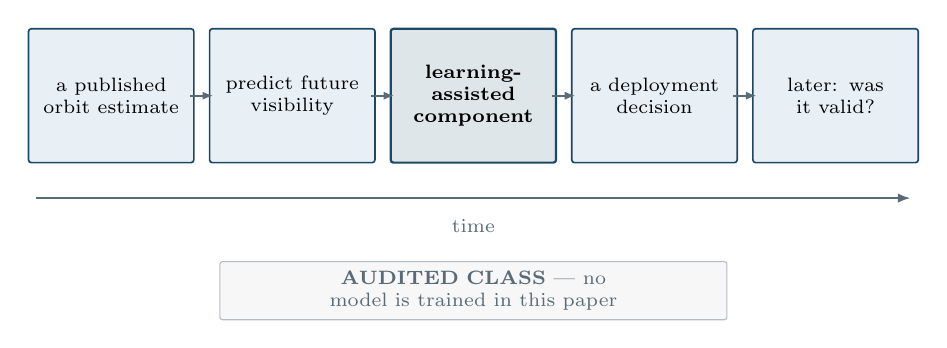
\begin{tikzpicture}[x=1mm,y=1mm]
    % one horizontal pipeline across the canvas: the shape reads in a glance, left to right
    \foreach \xx/\lab in {%
        0/{a published orbit estimate},
        23/{predict future visibility},
        69/{a deployment decision},
        92/{later: was it valid?}}
      \node[tnode,text width=19mm,minimum height=17mm,align=center,font=\scriptsize] at (\xx,0)
        {\lab};
    \node[tnode,text width=19mm,minimum height=17mm,align=center,font=\scriptsize,
          fill=oeaccent!14,draw=oeaccent,line width=0.8pt] at (46,0)
      {\textbf{learning-assisted component}};
    \foreach \aa/\bb in {0/23,23/46,46/69,69/92}
      \draw[flow,line width=0.8pt] (\aa+10,0) -- (\bb-10,0);
    \draw[oegrey,line width=0.7pt,-{Latex[length=1.6mm]}] (-9.5,-13) -- (101.5,-13);
    \node[font=\scriptsize,text=oegrey,anchor=north] at (46,-14.5) {time};
    \node[draw=oegrey!45,fill=black!3,rounded corners=1pt,line width=0.4pt,inner sep=1.2mm,
          font=\scriptsize,text=oegrey,align=center,text width=62mm,anchor=north] at (46,-21)
      {\textbf{AUDITED CLASS} --- no model is trained in this paper};
  \end{tikzpicture}
  \punch{The model may use only orbit information that existed at decision time.}
\end{frame}

% 3 ---------------------------------------------------------------- where the input comes from
% "element set" was previously an alias in scare quotes. Here it is taught: who produces it, what it
% is, and why it keeps being replaced -- all three are load-bearing later.
\begin{frame}{Where the orbital-state records come from}
  \centering
  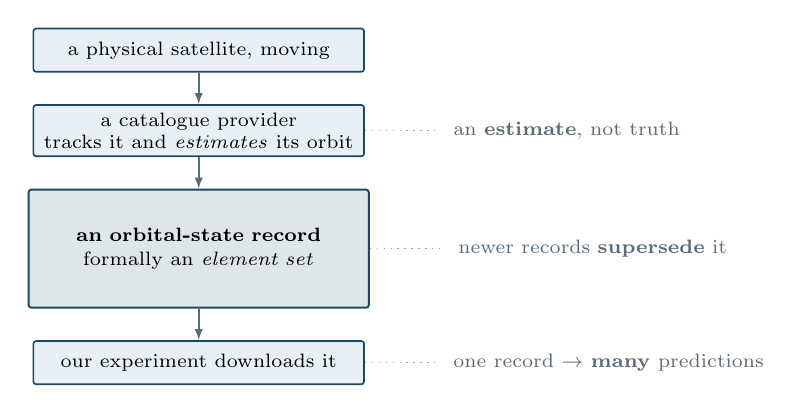
\begin{tikzpicture}[x=1mm,y=1mm]
    % one vertical source path; every note is tied to its node by a leader
    \node[tnode,text width=40mm,anchor=north] (s) at (0,34) {a physical satellite, moving};
    \node[tnode,text width=40mm,anchor=north] (tr) at ([yshift=-4mm]s.south)
      {a catalogue provider\\ tracks it and \emph{estimates} its orbit};
    \node[card,text width=40mm,anchor=north,fill=oeaccent!14] (r) at ([yshift=-4mm]tr.south)
      {\textbf{an orbital-state record}\\[0.1em]{\scriptsize formally an \emph{element set}}};
    \node[tnode,text width=40mm,anchor=north] (dl) at ([yshift=-4mm]r.south)
      {our experiment downloads it};
    \foreach \sa/\tb in {s/tr,tr/r,r/dl} \draw[flow] (\sa.south) -- (\tb.north);
    \foreach \nd/\note in {%
        tr/{an \textbf{estimate}, not truth},
        r/{newer records \textbf{supersede} it},
        dl/{one record $\to$ \textbf{many} predictions}}
      {\draw[oegrey!60,dotted,line width=0.5pt] (\nd.east) -- ([xshift=9mm]\nd.east);
       \node[font=\scriptsize,text=oegrey,anchor=west,align=left,text width=40mm]
         at ([xshift=10mm]\nd.east) {\note};}
  \end{tikzpicture}
  \punch{Each orbital-state record is an estimate that may later be superseded.}
\end{frame}

% 4 ---------------------------------------------------------------- propagation and passes
% Both terms are defined here, physically: propagation is what turns one record into future
% positions, and a pass is when the satellite is above the horizon for a ground station. The
% parent-to-many-children shape taught here is what L4.7 later tests.
\begin{frame}{One record, many predicted passes}
  \centering
  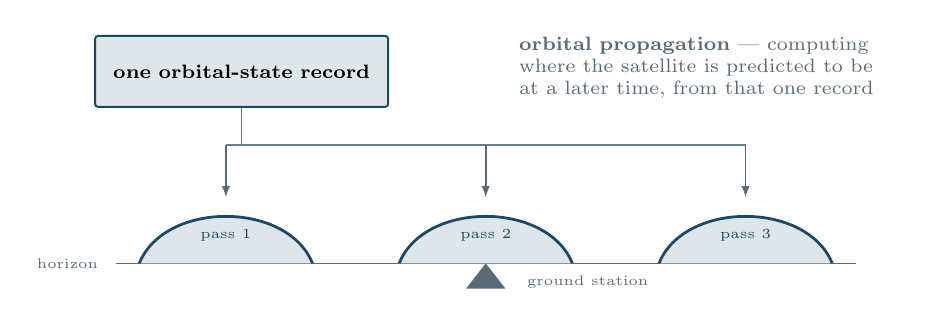
\begin{tikzpicture}[x=1mm,y=1mm]
    \node[card,text width=34mm,minimum height=9mm,fill=oeaccent!14,anchor=north] (rec) at (16,29)
      {\textbf{one orbital-state record}};
    \node[font=\scriptsize,text=oegrey,anchor=north west,align=left,text width=48mm] at (50,30)
      {\textbf{orbital propagation} --- computing where the satellite is predicted to be at a
       later time, from that one record};
    % spine, then one vertical drop per predicted window
    \draw[oeaccent!70,line width=0.6pt] (rec.south) -- (16,15) -- (14,15) -- (80,15);
    \foreach \cx in {14,47,80} \draw[flow] (\cx,15) -- (\cx,8.4);
    % horizon, ground station, three visibility windows
    \draw[oegrey,line width=0.6pt] (0,0) -- (94,0);
    \node[font=\tiny,text=oegrey,anchor=east] at (-1,0) {horizon};
    \fill[oegrey] (47,0) -- (44.5,-3.2) -- (49.5,-3.2) -- cycle;
    \node[font=\tiny,text=oegrey,anchor=west] at (51,-2.4) {ground station};
    \foreach \cx/\nn in {14/1,47/2,80/3}
      {\fill[oeaccent!14] (\cx-11,0) to[out=68,in=112] (\cx+11,0) -- cycle;
       \draw[oeaccent,line width=1.0pt] (\cx-11,0) to[out=68,in=112] (\cx+11,0);
       \node[font=\tiny,text=oeaccent] at (\cx,3.6) {pass \nn};}
  \end{tikzpicture}
  \punch{A \emph{pass} is one interval when the satellite is predicted to be visible from the
         ground station.}
  \par\vspace{-0.2em}
  {\scriptsize\color{oegrey}\hfill The orbit repeats, so the satellite returns over the same ground
   station again and again --- one record therefore predicts many passes.\hfill}
\end{frame}

% 5 ---------------------------------------------------------------- the two clocks
% Named explicitly, because the whole availability failure is the gap between them.
\begin{frame}{Two clocks, and a decision between them}
  \centering
  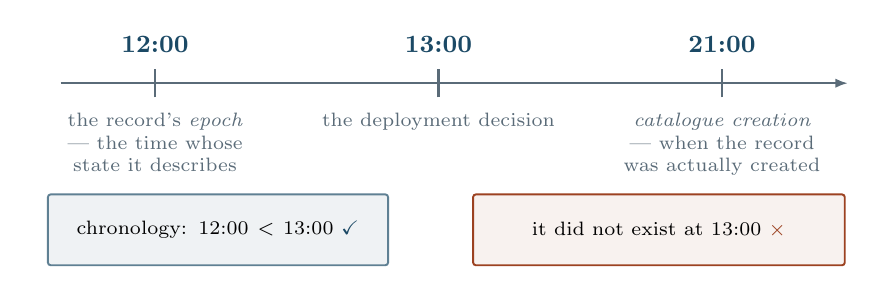
\begin{tikzpicture}[x=1mm,y=1mm]
    \draw[oegrey,line width=0.8pt,-{Latex[length=1.6mm]}] (0,14) -- (100,14);
    \foreach \x/\lab/\sub in {12/12:00/{the record's \emph{epoch} --- the time whose state it
                                        describes},
                              48/13:00/{the deployment decision},
                              84/21:00/{\emph{catalogue creation} --- when the record was actually
                                        created}}
      {\draw[oegrey,line width=0.8pt] (\x,12.2) -- (\x,15.8);
       \node[font=\small\bfseries,color=oeaccent,anchor=south] at (\x,16.6) {\lab};
       \node[font=\scriptsize,color=oegrey,anchor=north,align=center,text width=30mm]
         at (\x,11.4) {\sub};}
    \node[cardgood,text width=40mm,minimum height=9mm,anchor=north] at (20,0)
      {chronology: $12{:}00 < 13{:}00$ \tick{\checkmark}};
    \node[cardbad,text width=44mm,minimum height=9mm,anchor=north] at (76,0)
      {it did not exist at $13{:}00$ \cross{$\times$}};
  \end{tikzpicture}
  \punch{The record describes the past, but did not exist yet at the decision.}
  \par\vspace{-0.2em}
  {\scriptsize\color{oegrey}\hfill A chronological split sees $12{:}00<13{:}00$ and treats the record
   as historical input. Catalogue creation trails the epoch by a per-satellite median of
   \Nlagmedian{}\,h across \Nlagobjects{} satellites.\hfill}
\end{frame}

\begin{frame}{What a chronological split can see}
  \centering
  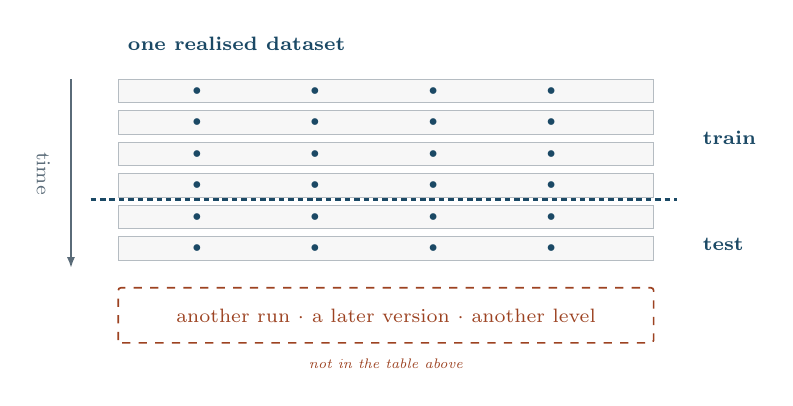
\begin{tikzpicture}[x=1mm,y=1mm]
    \node[hdr,anchor=west] at (12,38) {one realised dataset};
    \foreach \i in {0,...,5}{
      \draw[draw=oegrey!45,fill=black!3,line width=0.3pt]
        (12,30.5-4*\i) rectangle (80,33.5-4*\i);
      \foreach \x in {22,37,52,67}
        \node[font=\tiny,color=oeaccent] at (\x,32-4*\i) {$\bullet$};}
    \draw[oeaccent,line width=1.2pt,dash pattern=on 2pt off 1.4pt] (8.5,18.2) -- (83,18.2);
    \node[hdr,anchor=west] at (85,26) {train};
    \node[hdr,anchor=west] at (85,12.5) {test};
    \draw[oegrey,line width=0.7pt,-{Latex[length=1.4mm]}] (6,33.5) -- (6,9.5);
    \node[font=\scriptsize,color=oegrey,rotate=-90] at (2.5,21.5) {time};
    \draw[oewarn,dashed,line width=0.6pt,rounded corners=1pt] (12,0) rectangle (80,7);
    \node[font=\scriptsize,text=oewarn,align=center] at (46,3.5)
      {another run $\cdot$ a later version $\cdot$ another level};
    \node[font=\tiny\itshape,text=oewarn,anchor=north] at (46,-0.8) {not in the table above};
  \end{tikzpicture}
  \punch{What if the counterexample is \emph{not} a row in this table?}
\end{frame}

% 6 ---------------------------------------------------------------- generalise to four cards
\begin{frame}{Four questions a split cannot answer}
  \centering
  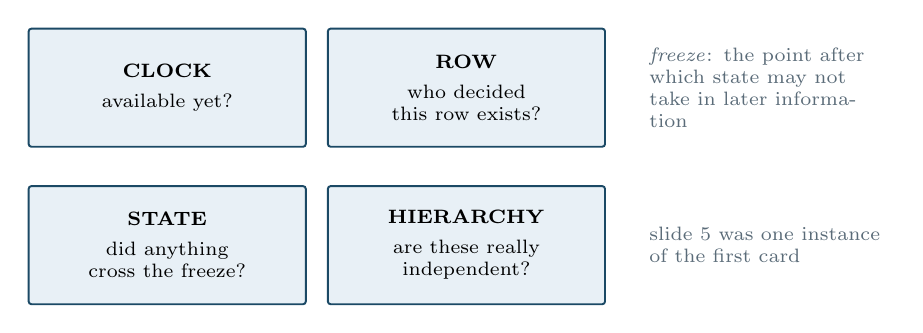
\begin{tikzpicture}[x=1mm,y=1mm]
    \node[card] at (0,20)  {\textbf{CLOCK}\\[0.35em] available yet?};
    \node[card] at (38,20) {\textbf{ROW}\\[0.35em] who decided this row exists?};
    \node[card] at (0,0)   {\textbf{STATE}\\[0.35em] did anything cross the freeze?};
    \node[card] at (38,0)  {\textbf{HIERARCHY}\\[0.35em] are these really independent?};
    \node[font=\scriptsize,color=oegrey,anchor=west,align=left,text width=30mm] at (60,20)
      {\emph{freeze}: the point after which state may not take in later information};
    \node[font=\scriptsize,color=oegrey,anchor=west,align=left,text width=30mm] at (60,0)
      {slide 5 was one instance of the first card};
  \end{tikzpicture}
  \punch{All four need evidence \emph{outside} one realised table.}
\end{frame}

% 7 ---------------------------------------------------------------- HERO FIGURE
\begin{frame}{Relational validity}
  \centering
  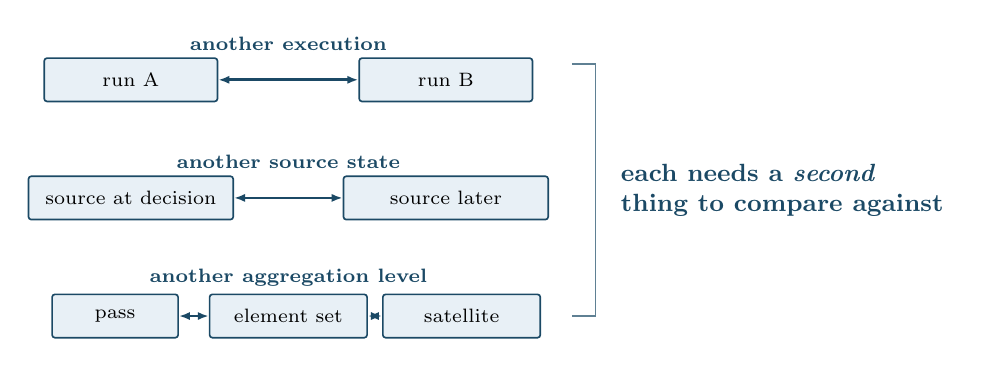
\begin{tikzpicture}[x=1mm,y=1mm]
    \node[tnode,text width=20mm] (ra) at (0,30) {run A};
    \node[tnode,text width=20mm] (rb) at (40,30) {run B};
    \draw[rel] (ra) -- (rb); \node[hdr,anchor=south] at (20,32.5) {another execution};

    \node[tnode,text width=24mm] (sa) at (0,15) {source at decision};
    \node[tnode,text width=24mm] (sb) at (40,15) {source later};
    \draw[rel] (sa) -- (sb); \node[hdr,anchor=south] at (20,17.5) {another source state};

    \node[tnode,text width=14mm] (p) at (-2,0) {pass};
    \node[tnode,text width=18mm] (e) at (20,0) {element set};
    \node[tnode,text width=18mm] (ob) at (42,0) {satellite};
    \draw[rel] (p) -- (e); \draw[rel] (e) -- (ob);
    \node[hdr,anchor=south] at (20,2.5) {another aggregation level};

    \draw[oeaccent!70,line width=0.6pt] (56,32) -- (59,32) -- (59,0) -- (56,0);
    \node[font=\small\bfseries,text=oeaccent,anchor=west,align=left,text width=42mm]
      at (61,16) {each needs a \emph{second} thing to compare against};
  \end{tikzpicture}
  \punch{The counterexample lives in a \emph{relation}, not in the table.}
\end{frame}

% ================================================================= ACT II -- what the tool is
% 8 ---------------------------------------------------------------- operational definition
\begin{frame}{What Orbit-Evidence does}
  \centering
  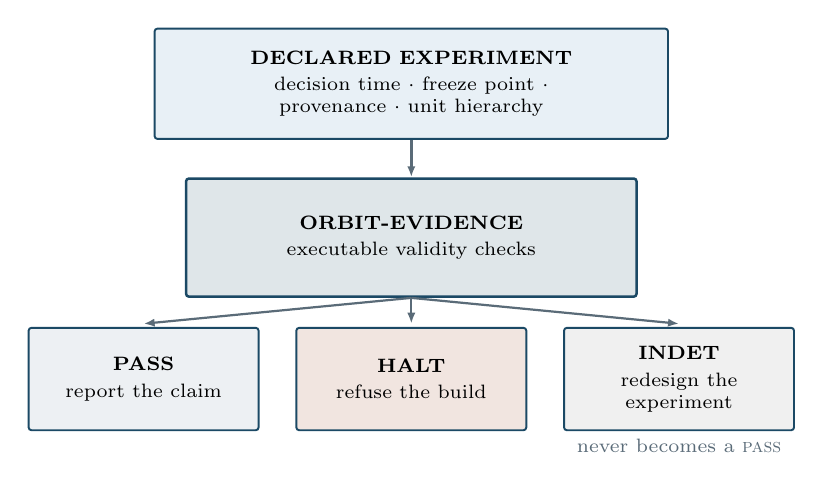
\begin{tikzpicture}[x=1mm,y=1mm]
    \node[card,text width=62mm,minimum height=14mm,anchor=north] (in) at (0,30)
      {\textbf{DECLARED EXPERIMENT}\\[0.2em]
       {\scriptsize decision time $\cdot$ freeze point $\cdot$ provenance $\cdot$ unit hierarchy}};
    \node[card,text width=54mm,minimum height=15mm,anchor=north,fill=oeaccent!14,
          draw=oeaccent,line width=0.9pt] (oe) at (0,11)
      {\textbf{ORBIT-EVIDENCE}\\[0.2em]{\scriptsize executable validity checks}};
    \draw[flow,line width=1.0pt] (in.south) -- (oe.north);
    \foreach \xx/\vd/\act/\fl in {%
        -34/{PASS}/{report the claim}/{oeaccent!8},
          0/{HALT}/{refuse the build}/{oewarn!14},
         34/{INDET}/{redesign the experiment}/{black!6}}
      {\node[card,text width=26mm,minimum height=13mm,anchor=north,fill=\fl] at (\xx,-8)
         {\textbf{\vd}\\[0.2em]{\scriptsize \act}};
       \draw[flow,line width=0.8pt] (oe.south) -- (\xx,-7.6);}
    \node[font=\scriptsize,text=oegrey,anchor=north] at (34,-21) {never becomes a \textsc{pass}};
  \end{tikzpicture}
  \punch{Can this experiment support the claim?}
\end{frame}

% 9 ---------------------------------------------------------------- method as four steps
\begin{frame}{The method, in four steps}
  \centering
  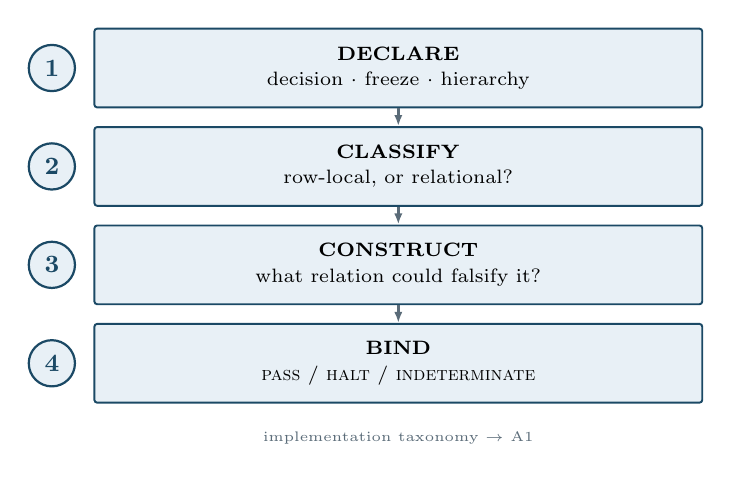
\begin{tikzpicture}[x=1mm,y=1mm]
    \foreach \i/\yy/\lab/\sub in {%
      1/26/DECLARE/{decision $\cdot$ freeze $\cdot$ hierarchy},
      2/13.5/CLASSIFY/{row-local, or relational?},
      3/1/CONSTRUCT/{what relation could falsify it?},
      4/-11.5/BIND/{\textsc{pass} / \textsc{halt} / \textsc{indeterminate}}}
      {\node[circle,draw=oeaccent,line width=0.8pt,fill=oelight,inner sep=1.1mm,
             font=\small\bfseries,text=oeaccent] (c\i) at (-44,\yy) {\i};
       \node[card,text width=74mm,minimum height=10mm,align=center] (s\i) at (0,\yy)
         {\textbf{\lab}\\[0.15em]{\scriptsize \sub}};}
    \foreach \aa/\bb in {1/2,2/3,3/4} \draw[flow,line width=0.9pt] (s\aa.south) -- (s\bb.north);
    \node[font=\tiny,text=oegrey,anchor=north] at (0,-19) {implementation taxonomy $\to$ A1};
  \end{tikzpicture}
  \punch{Every step is declared before the data is touched.}
\end{frame}

% ================================================================= ACT III -- the two checks
% 10 --------------------------------------------------------------- L4.6 impossible vs relational
\begin{frame}{Can the provenance declaration be trusted?}
  \ruletag{\rulename{L4.6}}
  \centering
  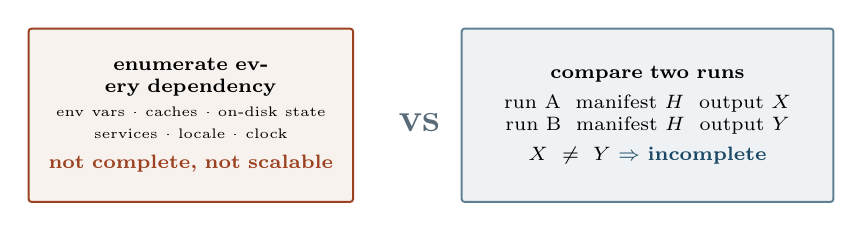
\begin{tikzpicture}[x=1mm,y=1mm]
    \node[cardbad,text width=38mm,minimum height=22mm,anchor=north] at (16,32)
      {\textbf{enumerate every dependency}\\[0.35em]
       {\tiny env vars · caches · on-disk state\\ services · locale · clock}\\[0.35em]
       \cross{not complete, not scalable}};
    \node[cardgood,text width=44mm,minimum height=22mm,anchor=north] at (74,32)
      {\textbf{compare two runs}\\[0.35em]
       {\scriptsize run A\ \ manifest $H$\ \ output $X$\\ run B\ \ manifest $H$\ \ output $Y$}\\[0.35em]
       $X \neq Y$ \tick{$\Rightarrow$ incomplete}};
    \node[font=\Large\bfseries,color=oegrey] at (45,20) {vs};
  \end{tikzpicture}
  \punch{We do not prove completeness. We make incompleteness \emph{falsifiable}.}
  \notclaim{that agreement certifies completeness --- it is consistent with an untested dependency.}
\end{frame}

% 11 --------------------------------------------------------------- L4.6 evidence state
\begin{frame}{How strong is the evidence for that check?}
  \ruletag{\rulename{L4.6}}
  \centering
  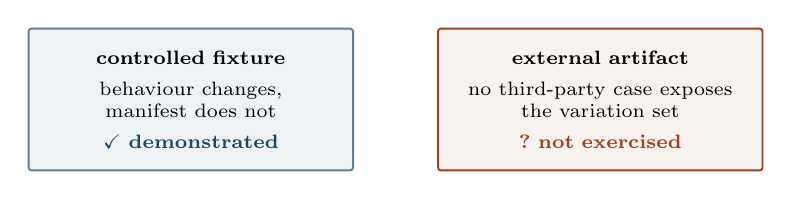
\begin{tikzpicture}[x=1mm,y=1mm]
    \node[cardgood,text width=38mm,minimum height=18mm] (a) at (0,10)
      {\textbf{controlled fixture}\\[0.4em] behaviour changes,\\manifest does not\\[0.4em]
       \tick{\checkmark\ demonstrated}};
    \node[cardbad,text width=38mm,minimum height=18mm] (b) at (52,10)
      {\textbf{external artifact}\\[0.4em] no third-party case exposes\\the variation set\\[0.4em]
       \cross{?\ not exercised}};
  \end{tikzpicture}
  \vfill

  {\footnotesize\color{oeaccent}\textbf{Advisor decision:} does the workshop need an
   independent external \rulename{L4.6} case?}
  \vspace{2em}
\end{frame}

% 12 --------------------------------------------------------------- L4.7 the modelling question
\begin{frame}{Are these really independent samples?}
  \ruletag{\rulename{L4.7}}
  \centering
  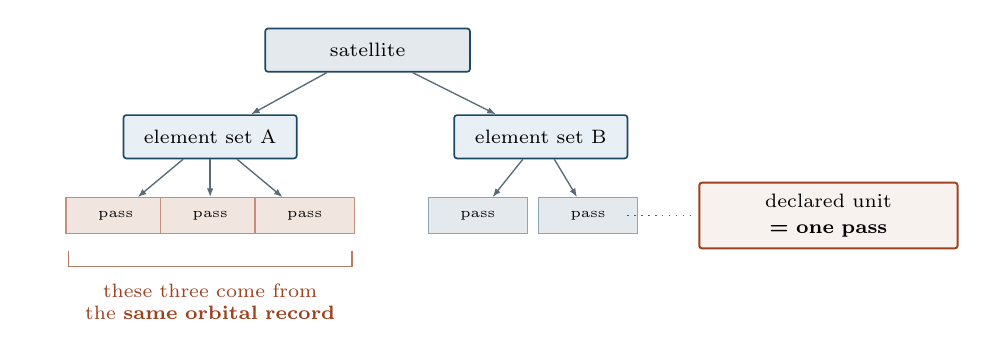
\begin{tikzpicture}[x=1mm,y=1mm]
    \node[tnode,text width=24mm,fill=oeaccent!12] (o) at (30,24) {satellite};
    \node[tnode,text width=20mm] (ea) at (10,13) {element set A};
    \node[tnode,text width=20mm] (eb) at (52,13) {element set B};
    \draw[tree] (o) -- (ea); \draw[tree] (o) -- (eb);
    \foreach \x/\n in {-2/1,10/2,22/3}
      \node[tleaf,fill=oewarn!14,draw=oewarn!60] (pa\n) at (\x,3) {pass};
    \foreach \x/\n in {44/4,58/5}
      \node[tleaf,fill=oeaccent!12,draw=oeaccent!50] (pb\n) at (\x,3) {pass};
    \draw[oewarn!70,line width=0.5pt] (-8,-1.5) -- (-8,-3.5) -- (28,-3.5) -- (28,-1.5);
    \node[font=\scriptsize,text=oewarn,anchor=north,align=center,text width=44mm] at (10,-4.5)
      {these three come from the \textbf{same orbital record}};
    \foreach \n in {1,2,3} \draw[tree] (ea) -- (pa\n);
    \foreach \n in {4,5} \draw[tree] (eb) -- (pb\n);
    \node[draw=oewarn,line width=0.7pt,fill=oewarn!7,rounded corners=1pt,inner sep=1.4mm,
          font=\scriptsize,align=center,anchor=west,text width=30mm] at (72,3)
      {declared unit\\[0.2em]\textbf{= one pass}};
    \draw[oewarn,dotted,line width=0.5pt] (63,3) -- (71,3);
  \end{tikzpicture}
  \punch{If the passes are dependent, why would aggregating create independence?}
  \par\vspace{-0.2em}
  \begin{center}\begin{minipage}{0.94\textwidth}\centering\scriptsize\color{oeaccent}
  Every pass propagated from one record inherits that record's estimation error: if the parent
  estimate is displaced, its passes move together.
  \end{minipage}\end{center}
\end{frame}

% 13 --------------------------------------------------------------- L4.7 permutation as a picture
\begin{frame}{The test: shuffle values, keep the groups}
  \centering
  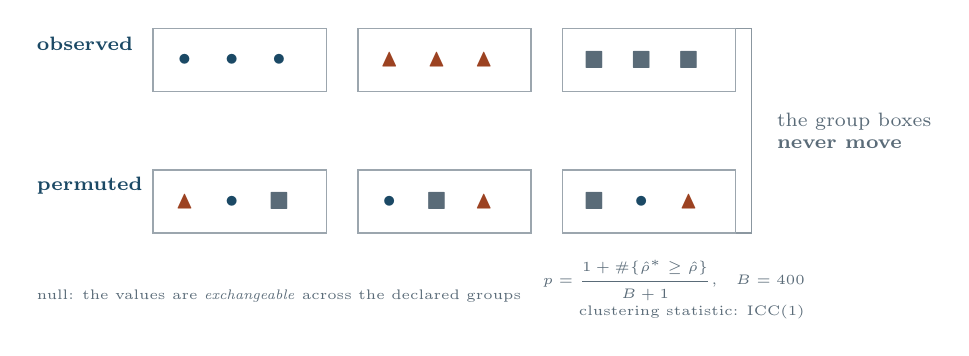
\begin{tikzpicture}[x=1mm,y=1mm]
    \node[hdr,anchor=west] at (0,26) {observed};
    \foreach \g in {0,1,2}{
      \draw[draw=oegrey!60,line width=0.5pt] (16+26*\g,20) rectangle (38+26*\g,28);}
    \foreach \x/\s in {20/$\bullet$,26/$\bullet$,32/$\bullet$} \node[font=\small,color=oeaccent] at (\x,24) {\s};
    \foreach \x/\s in {46/$\blacktriangle$,52/$\blacktriangle$,58/$\blacktriangle$} \node[font=\small,color=oewarn] at (\x,24) {\s};
    \foreach \x/\s in {72/$\blacksquare$,78/$\blacksquare$,84/$\blacksquare$} \node[font=\small,color=oegrey] at (\x,24) {\s};

    \node[hdr,anchor=west] at (0,8) {permuted};
    \foreach \g in {0,1,2}{
      \draw[draw=oegrey!60,line width=0.5pt] (16+26*\g,2) rectangle (38+26*\g,10);}
    \foreach \x/\s/\c in {20/$\blacktriangle$/oewarn,26/$\bullet$/oeaccent,32/$\blacksquare$/oegrey,
                          46/$\bullet$/oeaccent,52/$\blacksquare$/oegrey,58/$\blacktriangle$/oewarn,
                          72/$\blacksquare$/oegrey,78/$\bullet$/oeaccent,84/$\blacktriangle$/oewarn}
      \node[font=\small,color=\c] at (\x,6) {\s};
    \draw[oegrey!70,line width=0.5pt] (90,28) -- (92,28) -- (92,2) -- (90,2);
    \node[font=\scriptsize,text=oegrey,anchor=west,align=left] at (94,15)
      {the group boxes\\ \textbf{never move}};
    \node[font=\tiny,color=oegrey,anchor=east] at (100,-4)
      {$p=\dfrac{1+\#\{\hat{\rho}^{*}\ge\hat{\rho}\}}{B+1}$,\quad $B=\NpermB$};
    \node[font=\tiny,text=oegrey,anchor=west] at (0,-6)
      {null: the values are \emph{exchangeable} across the declared groups};
    \node[font=\tiny,text=oegrey,anchor=east] at (100,-8)
      {clustering statistic: ICC(1)};
  \end{tikzpicture}
  \punch{Only the values move. The grouping is held fixed.}
  \notclaim{a variance share --- the ICC is used here as a \emph{clustering statistic}.}
\end{frame}

% 14 --------------------------------------------------------------- INDETERMINATE, two stages
\begin{frame}{A design can be too small to test at all}
  \centering
  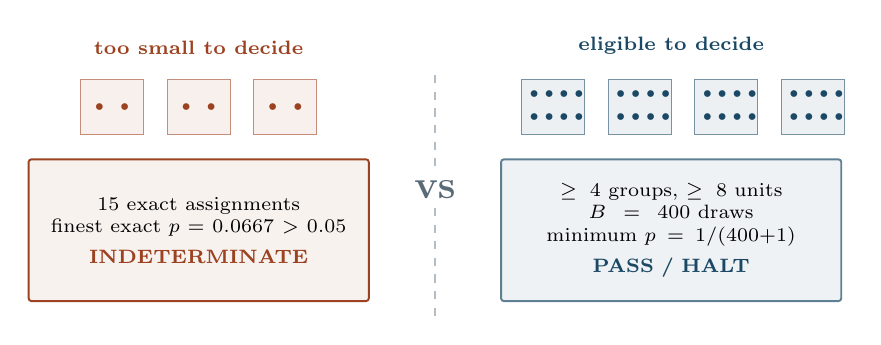
\begin{tikzpicture}[x=1mm,y=1mm]
    % the two designs, drawn: groups are boxes, units are dots
    \node[hdr,anchor=south,text=oewarn] at (16,36) {too small to decide};
    \foreach \g in {0,1,2}{
      \draw[draw=oewarn!60,fill=oewarn!8,line width=0.4pt]
        (1+11*\g,27) rectangle (9+11*\g,34);
      \foreach \u in {0,1}
        \node[font=\tiny,text=oewarn] at (3.4+11*\g+3.2*\u,30.5) {$\bullet$};}
    \node[hdr,anchor=south,text=oeaccent] at (76,36) {eligible to decide};
    \foreach \g in {0,1,2,3}{
      \draw[draw=oeaccent!60,fill=oeaccent!8,line width=0.4pt]
        (57+11*\g,27) rectangle (65+11*\g,34);
      \foreach \u in {0,1,2,3}{
        \node[font=\tiny,text=oeaccent] at (58.6+11*\g+1.9*\u,32.2) {$\bullet$};
        \node[font=\tiny,text=oeaccent] at (58.6+11*\g+1.9*\u,29.2) {$\bullet$};}}
    \node[cardbad,text width=40mm,minimum height=18mm,anchor=north] at (16,24)
      {{\scriptsize $\Nassignthree$ exact assignments\\
        finest exact $p=\Nminpthree > \Nalpha$}\\[0.4em]
       \cross{INDETERMINATE}};
    \node[cardgood,text width=40mm,minimum height=18mm,anchor=north] at (76,24)
      {{\scriptsize $\ge\Nmingroups$ groups, $\ge\Nminunits$ units\\
        $B=\NpermB$ draws\\ minimum $p=1/(\NpermB{+}1)$}\\[0.4em]
       \tick{PASS / HALT}};
    \draw[oegrey!45,line width=0.5pt,dashed] (46,4) -- (46,35);
    \node[font=\Large\bfseries,text=oegrey,fill=white,inner sep=0.8mm] at (46,20) {vs};
  \end{tikzpicture}
  \punch{Exact geometry decides eligibility; sampling decides the rest.}
\end{frame}

% 15 --------------------------------------------------------------- the tradeoff, named
% L4.6 and L4.7 each relax an uncertifiable question into a refutable one. Shown separately they
% look like two local design choices; named together they are the deck's design principle, and the
% first question a reviewer asks ("did you swap the hard problem for an easier one?") is answered
% here rather than left implicit.
\begin{frame}{The tradeoff is deliberate}
  \centering
  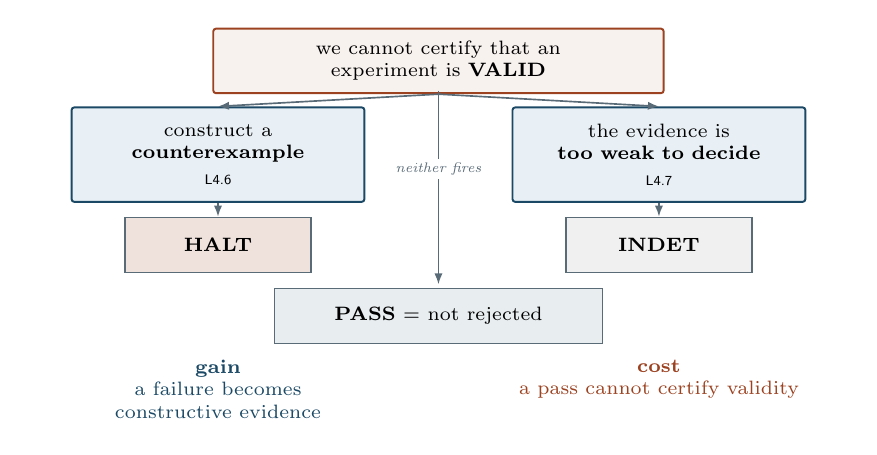
\begin{tikzpicture}[x=1mm,y=1mm]
    \node[cardbad,text width=54mm,minimum height=8mm,anchor=north] (top) at (28,30)
      {we cannot certify that an experiment is \textbf{VALID}};
    \node[card,text width=34mm,minimum height=12mm,anchor=north] (lf) at (0,20)
      {construct a\\ \textbf{counterexample}\\[0.15em] {\tiny \rulename{L4.6}}};
    \node[card,text width=34mm,minimum height=12mm,anchor=north] (rt) at (56,20)
      {the evidence is\\ \textbf{too weak to decide}\\[0.15em] {\tiny \rulename{L4.7}}};
    \draw[flow] (top.south) -- (lf.north);
    \draw[flow] (top.south) -- (rt.north);
    \node[chip,text width=22mm,fill=oewarn!16,anchor=north] (hl) at (0,6) {\textbf{HALT}};
    \node[chip,text width=22mm,fill=black!6,anchor=north] (id) at (56,6) {\textbf{INDET}};
    \draw[flow] (lf.south) -- (hl.north);
    \draw[flow] (rt.south) -- (id.north);
    \draw[flow] (28,22) -- (28,-2.6);
    \node[font=\tiny\itshape,text=oegrey,fill=white,inner sep=0.5mm] at (28,12)
      {neither fires};
    \node[chip,text width=40mm,fill=oeaccent!10,anchor=north] at (28,-3)
      {\textbf{PASS} $=$ not rejected};
    \node[font=\scriptsize,text=oeaccent,anchor=north,align=center,text width=46mm] at (0,-11)
      {\textbf{gain}\\ a failure becomes\\ constructive evidence};
    \node[font=\scriptsize,text=oewarn,anchor=north,align=center,text width=46mm] at (56,-11)
      {\textbf{cost}\\ a pass cannot certify validity};
  \end{tikzpicture}
  \punch{We trade certification for falsifiability and honest abstention.}
\end{frame}

% ================================================================= ACT IV -- evidence
% 15 --------------------------------------------------------------- curated regression, as bars
\begin{frame}{A chronological baseline misses most represented faults}
  \centering
  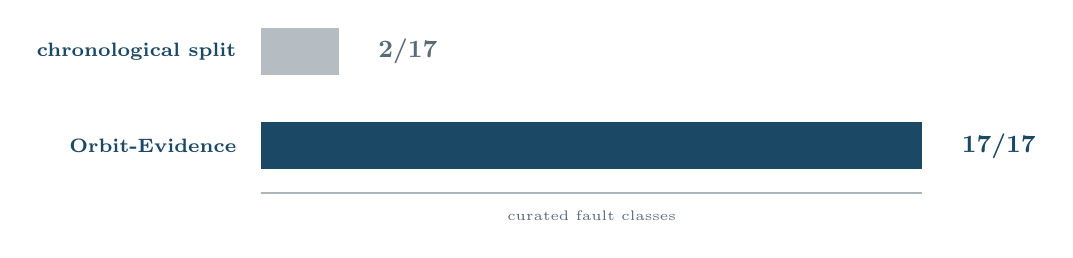
\begin{tikzpicture}[x=1.9mm,y=1mm]
    \node[hdr,anchor=east] at (-1,18) {chronological split};
    \fill[barlo] (0,15) rectangle (\Nchrono*2.6,21);
    \node[font=\small\bfseries,color=oegrey,anchor=west] at (\Nchrono*2.6+2,18) {\Nchrono/\Nfaults};
    \node[hdr,anchor=east] at (-1,6) {Orbit-Evidence};
    \fill[bar] (0,3) rectangle (\Ncontract*2.6,9);
    \node[font=\small\bfseries,color=oeaccent,anchor=west] at (\Ncontract*2.6+2,6) {\Ncontract/\Nfaults};
    \draw[oegrey!50,line width=0.4pt] (0,0) -- (\Nfaults*2.6,0);
    \node[font=\tiny,color=oegrey,anchor=north] at (\Nfaults*1.3,-1) {curated fault classes};
  \end{tikzpicture}
  \vspace{0.3em}


  \notclaim{a detector benchmark --- differing \emph{scope}: the baseline tests ordering, and
   this is represented-fault regression reachability.}
\end{frame}

% 16 --------------------------------------------------------------- operating characteristic
\begin{frame}{How does the gate behave as dependence grows?}
  \ruletag{\rulename{L4.7} --- one registered design}
  \centering
  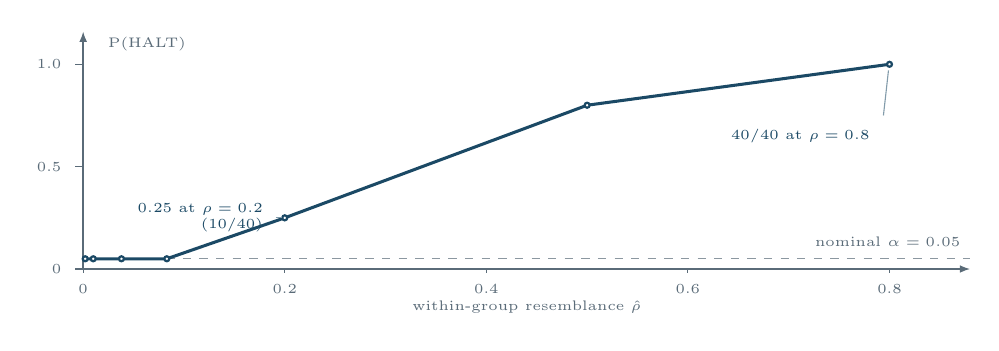
\begin{tikzpicture}[x=1.28mm,y=26mm]
    \draw[oegrey,line width=0.5pt,-{Latex[length=1.3mm]}] (0,0) -- (88,0);
    \draw[oegrey,line width=0.5pt,-{Latex[length=1.3mm]}] (0,0) -- (0,1.16);
    \foreach \x/\lab in {0/0, 20/0.2, 40/0.4, 60/0.6, 80/0.8}
      {\draw[oegrey] (\x,0) -- (\x,-0.02); \node[below,font=\tiny,color=oegrey] at (\x,-0.03) {\lab};}
    \foreach \y/\lab in {0/0, 0.5/0.5, 1/1.0}
      {\draw[oegrey] (0,\y) -- (-0.8,\y); \node[left,font=\tiny,color=oegrey] at (-1.2,\y) {\lab};}
    \draw[dashed,oegrey!70,line width=0.4pt] (0,0.05) -- (88,0.05);
    \node[font=\tiny,color=oegrey,anchor=south east] at (88,0.06) {nominal $\alpha=\Nalpha$};
    \draw[oeaccent,line width=1.1pt]
      (0.2,0.05) -- (1,0.05) -- (3.8,0.05) -- (8.3,0.05) -- (20,0.25) -- (50,0.8) -- (80,1.0);
    \foreach \x/\y in {0.2/0.05, 1/0.05, 3.8/0.05, 8.3/0.05, 20/0.25, 50/0.8, 80/1.0}
      \draw[fill=white,draw=oeaccent,line width=0.8pt] (\x,\y) circle (0.9pt);
    \draw[oeaccent!55,line width=0.4pt] (19.1,0.25) -- (19.7,0.25);
    \node[font=\tiny,color=oeaccent,anchor=east,align=right] at (18.8,0.25)
      {$\Npowerlo$ at $\rho=\Nrholo$\\({\Nhaltslo}/{\Nseeds})};
    \draw[oeaccent!55,line width=0.4pt] (79.4,0.75) -- (79.9,0.97);
    \node[font=\tiny,color=oeaccent,anchor=north east,align=right] at (79,0.73)
      {$\Nhaltshi/\Nseeds$ at $\rho=\Nrhohi$};
    \node[below,font=\tiny,color=oegrey] at (44,-0.11) {within-group resemblance $\hat{\rho}$};
    \node[font=\tiny,color=oegrey,anchor=west] at (1.5,1.10) {P(HALT)};
  \end{tikzpicture}
  \vspace{-0.1em}

  {\footnotesize \Ncalgroups{} groups $\times$ \Ncalunits{} units. Clean:
   $\Ncleanhalts/\Ncleanpaths = \Nrate$, Wilson $[\Nwlo,\Nwhi]$.}
  \notclaim{transfer to the real-data geometries --- one registered design only.}
\end{frame}

% 17 --------------------------------------------------------------- real-data cohort
\begin{frame}{How much did a later update move the prediction?}
  \ruletag{the along-track \emph{update increment}}
  \centering
  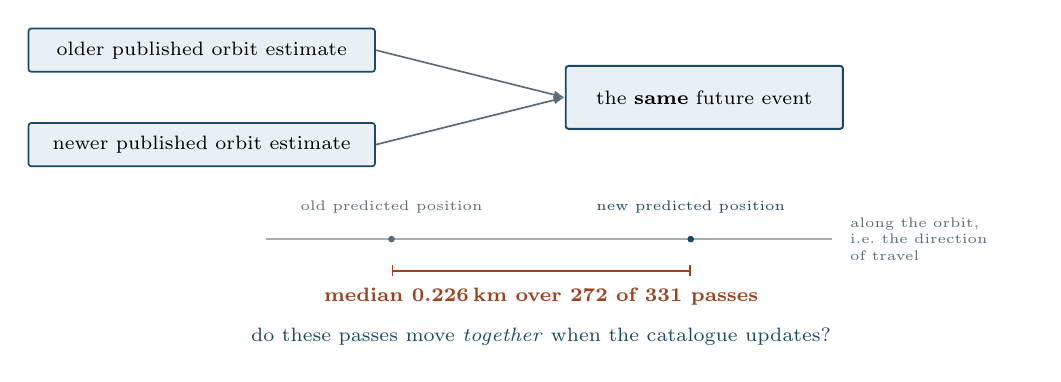
\begin{tikzpicture}[x=1mm,y=1mm]
    % panel 1 -- two published estimates, one future event
    \node[tnode,text width=42mm,anchor=east] (old) at (34,32) {older published orbit estimate};
    \node[tnode,text width=42mm,anchor=east] (new) at (34,20) {newer published orbit estimate};
    \node[card,text width=32mm,minimum height=8mm,anchor=west] (ev) at (58,26)
      {the \textbf{same} future event};
    \draw[flow] (old.east) -- (ev.west);
    \draw[flow] (new.east) -- (ev.west);
    % panel 2 -- where each estimate says that event will be
    \draw[oegrey!55,line width=0.5pt] (20,8) -- (92,8);
    \node[font=\tiny,text=oegrey,anchor=west,align=left,text width=22mm] at (93,8)
      {along the orbit, i.e.\ the direction of travel};
    \fill[oegrey]   (36,8) circle (1.2pt);
    \fill[oeaccent] (74,8) circle (1.2pt);
    \node[font=\tiny,text=oegrey,anchor=south]   at (36,10) {old predicted position};
    \node[font=\tiny,text=oeaccent,anchor=south] at (74,10) {new predicted position};
    \draw[{|[width=1.4mm]}-{|[width=1.4mm]},oewarn,line width=0.7pt] (36,4) -- (74,4);
    \node[font=\scriptsize\bfseries,text=oewarn,anchor=north] at (55,3)
      {median \Natmedian{}\,km over \Natused{} of \Npasses{} passes};
    \node[font=\scriptsize,text=oeaccent,anchor=north] at (55,-2)
      {do these passes move \emph{together} when the catalogue updates?};
  \end{tikzpicture}
  \punch{How far a later catalogue update moved the predicted pass.}
  \notclaim{position error against truth --- nothing here is compared to a true orbit.}
\end{frame}

% 18 --------------------------------------------------------------- real-data result, as hierarchy
\begin{frame}{Pooled: passes are not independent at any tested grouping}
  \ruletag{\rulename{L4.7} on real orbital data}
  \centering
  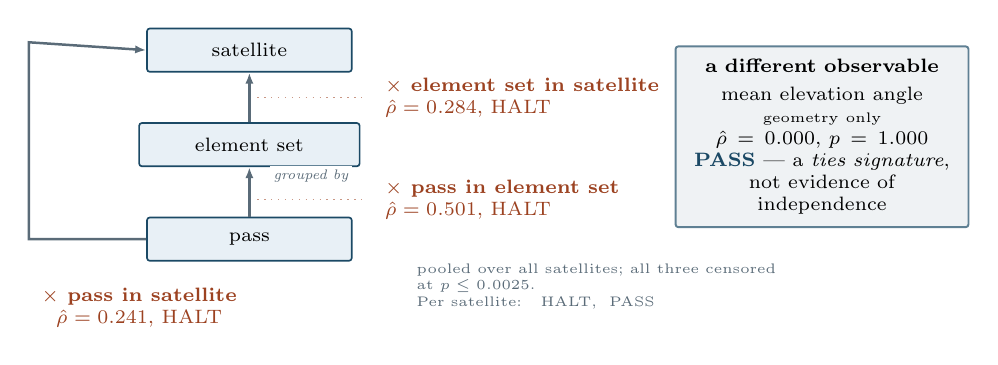
\begin{tikzpicture}[x=1mm,y=1mm]
    % satellite on top, matching slides 3 and 12; arrows point unit -> the grouping it is tested against
    \node[tnode,text width=24mm] (o) at (26,23) {satellite};
    \node[tnode,text width=26mm] (e) at (26,11) {element set};
    \node[tnode,text width=24mm] (p) at (26,-1) {pass};
    \draw[flow,line width=0.9pt] (p) -- (e);
    \draw[flow,line width=0.9pt] (e) -- (o);
    \node[font=\tiny\itshape,text=oegrey,anchor=west,fill=white,inner sep=0.5mm] at (28.5,7)
      {grouped by};
    \draw[oewarn!55,dotted,line width=0.5pt] (27,4) -- (41,4);
    \draw[oewarn!55,dotted,line width=0.5pt] (27,17) -- (41,17);
    \node[font=\scriptsize,text=oewarn,anchor=west,align=left] at (42,4)
      {\textbf{$\times$ pass in element set}\\ $\hat{\rho}=\Naticc$, HALT};
    \node[font=\scriptsize,text=oewarn,anchor=west,align=left] at (42,17)
      {\textbf{$\times$ element set in satellite}\\ $\hat{\rho}=\Naticcelset$, HALT};
    % cross edge: pass grouped by satellite, routed left as a polyline with known geometry
    \draw[flow,line width=0.9pt] (p.west) -- (-2,-1) -- (-2,24) -- (o.west);
    \node[font=\scriptsize,text=oewarn,anchor=north,align=center] at (12,-6)
      {\textbf{$\times$ pass in satellite}\\ $\hat{\rho}=\Naticcobj$, HALT};
    \node[cardgood,text width=34mm,minimum height=15mm,anchor=west] at (80,12)
      {\textbf{a different observable}\\[0.25em] mean elevation angle\\ {\tiny geometry only}\\
       $\hat{\rho}=\Nelevicc$, $p=\Nelevp$\\
       \tick{PASS} --- a \emph{ties signature},\\ not evidence of independence};
    \node[font=\tiny,text=oegrey,anchor=west,align=left,text width=46mm] at (46,-7)
      {pooled over all satellites; all three censored at $p\le\Natp$.\\
       Per satellite: \Nperobjhalt{} HALT, \Nperobjpass{} PASS};
  \end{tikzpicture}
  \punch{In the pooled analysis, independence is rejected at all three tested groupings.}
  \notclaim{a variance decomposition --- passes sharing an element set also share a satellite.}
\end{frame}

% 19 --------------------------------------------------------------- third-party verdict stack
\begin{frame}{The unchanged contract on a frozen third-party artifact}
  \ruletag{public spacecraft-anomaly \textsc{lstm} artifact, KDD 2018}
  \centering
  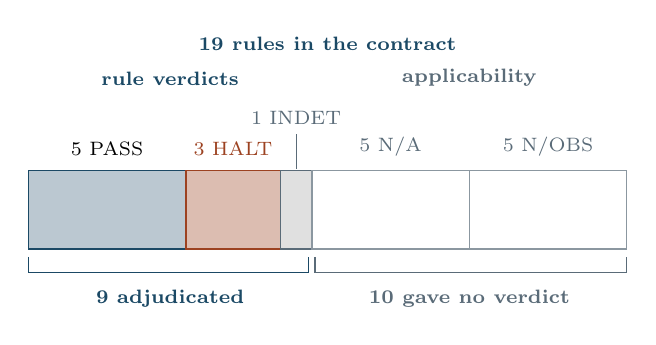
\begin{tikzpicture}[x=1mm,y=1mm]
    % one bar, 19 segments: the partition IS the figure, so no connector has to carry it
    \node[hdr,anchor=south] at (38,34) {\Nextrules{} rules in the contract};
    \node[hdr,anchor=south] at (18,29.5) {rule verdicts};
    \node[hdr,anchor=south,text=oegrey] at (56,29.5) {applicability};
    \draw[fill=oeaccent!30,draw=oeaccent,line width=0.5pt]  (0,10)  rectangle (20,20);
    \draw[fill=oewarn!35,draw=oewarn,line width=0.5pt]      (20,10) rectangle (32,20);
    \draw[fill=black!12,draw=oegrey,line width=0.5pt]       (32,10) rectangle (36,20);
    \draw[fill=white,draw=oegrey!70,line width=0.5pt]       (36,10) rectangle (56,20);
    \draw[fill=white,draw=oegrey!70,line width=0.5pt]       (56,10) rectangle (76,20);
    \node[font=\scriptsize,anchor=south] at (10,20.6) {\Nextpass{} PASS};
    \node[font=\scriptsize,anchor=south,text=oewarn] at (26,20.6) {\Nexthalt{} HALT};
    \node[font=\scriptsize,anchor=south,text=oegrey] at (46,20.6) {\Nextna{} N/A};
    \node[font=\scriptsize,anchor=south,text=oegrey] at (66,20.6) {\Nextnobs{} N/OBS};
    \draw[oegrey,line width=0.4pt] (34,24.6) -- (34,20.2);
    \node[font=\scriptsize,anchor=south,text=oegrey] at (34,24.6) {\Nextindet{} INDET};
    % the two dispositions, bracketed under the segments they cover
    \draw[oeaccent,line width=0.5pt] (0,9) -- (0,7) -- (35.6,7) -- (35.6,9);
    \draw[oegrey,line width=0.5pt] (36.4,9) -- (36.4,7) -- (76,7) -- (76,9);
    \node[font=\scriptsize\bfseries,text=oeaccent,anchor=north] at (18,6)
      {\Nextadjudicated{} adjudicated};
    \node[font=\scriptsize\bfseries,text=oegrey,anchor=north] at (56,6)
      {\Nextnoverdict{} gave no verdict};
  \end{tikzpicture}
  \punch{Not observable is never scored as compliance.}
\end{frame}

% 20 --------------------------------------------------------------- intervention before/after
\begin{frame}{Did train and validation share the same samples?}
  \ruletag{\rulename{L4.1} --- correcting it changed the decision}
  \centering
  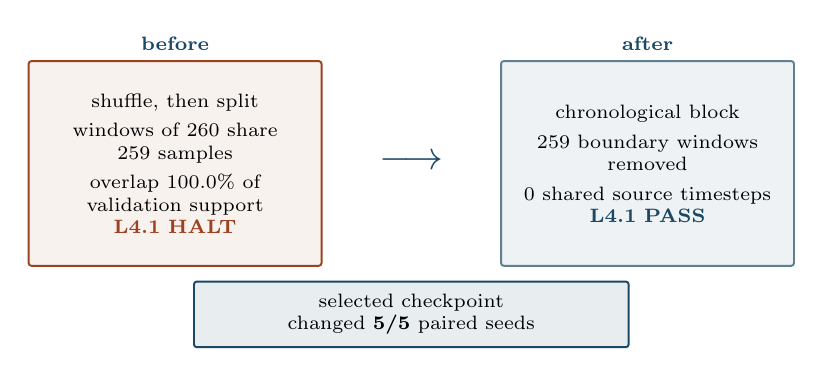
\begin{tikzpicture}[x=1mm,y=1mm]
    \node[hdr,anchor=south] at (18,28) {before};
    \node[hdr,anchor=south] at (78,28) {after};
    \node[cardbad,text width=34mm,minimum height=26mm,anchor=north] at (18,28)
      {shuffle, then split\\[0.35em]
       {\scriptsize windows of \Nwindowspan{} share\\ \Nboundarydropped{} samples}\\[0.35em]
       {\scriptsize overlap \Nconsoverlap\% of validation support}\\ \cross{L4.1 HALT}};
    \node[cardgood,text width=34mm,minimum height=26mm,anchor=north] at (78,28)
      {chronological block\\[0.35em]
       {\scriptsize \Nboundarydropped{} boundary windows\\ removed}\\[0.35em]
       {\scriptsize \Nconsoverlapcorr{} shared source timesteps}\\ \tick{L4.1 PASS}};
    \node[font=\Large\bfseries,color=oeaccent] at (48,15) {$\longrightarrow$};
    \node[card,text width=52mm,minimum height=8mm,fill=oeaccent!10,anchor=north] at (48,0)
      {selected checkpoint changed \textbf{\Nconschanged/\Nconsseeds} paired seeds};
  \end{tikzpicture}
  \notclaim{an accuracy improvement --- at \Nconsseeds{} seeds the smallest two-sided $p$ is
   $\Nconsminp$, so the downstream endpoint is \textbf{not estimable}.}
\end{frame}

% 22 --------------------------------------------------------------- how an engineer uses it
% The deck could show what the checker decides but never where an engineer puts it. Without this
% the verdict reads as commentary; with it, the verdict is a build outcome.
\begin{frame}{Where this sits in a real experiment}
  \centering
  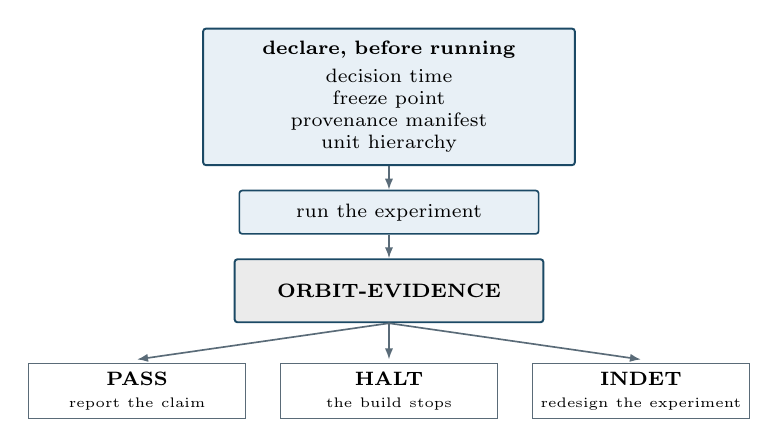
\begin{tikzpicture}[x=1mm,y=1mm]
    \node[card,text width=44mm,anchor=north] (dec) at (0,34)
      {\textbf{declare, before running}\\[0.25em]
       {\scriptsize decision time\\ freeze point\\ provenance manifest\\ unit hierarchy}};
    \node[tnode,text width=36mm,anchor=north] (run) at ([yshift=-3mm]dec.south)
      {run the experiment};
    \draw[flow] (dec.south) -- (run.north);
    \node[card,text width=36mm,minimum height=8mm,fill=black!8,anchor=north] (oe)
      at ([yshift=-3mm]run.south) {\textbf{ORBIT-EVIDENCE}};
    \draw[flow] (run.south) -- (oe.north);
    \foreach \xx/\lab/\act in {-32/PASS/{report the claim},
                                0/HALT/{the build stops},
                               32/INDET/{redesign the experiment}}
      {\node[chip,text width=26mm,anchor=north]
         at ([xshift=\xx mm,yshift=-5mm]oe.south) {\textbf{\lab}\\{\tiny \act}};
       \draw[flow] (oe.south) -- ([xshift=\xx mm,yshift=-4.6mm]oe.south);}
  \end{tikzpicture}
  \punch{The verdict is a build outcome, not a sentence in a paper.}
\end{frame}

% ================================================================= ACT V -- positioning
% 21 --------------------------------------------------------------- novelty as a conversion
\begin{frame}{Prior work supplies the primitives; we change what is tested}
  \centering
  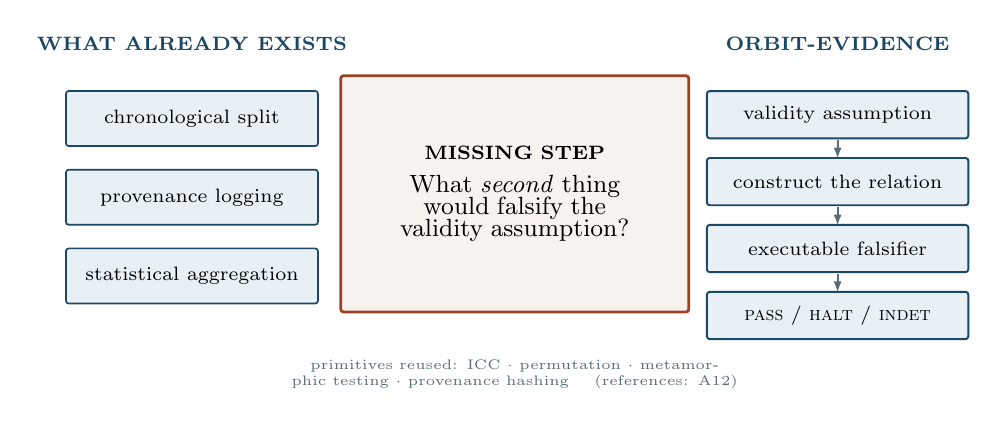
\begin{tikzpicture}[x=1mm,y=1mm]
    % three zones; the middle one is the point, so it is the biggest thing on the slide
    \node[hdr,anchor=north] at (13,40) {WHAT ALREADY EXISTS};
    \foreach \yy/\what in {32/{chronological split}, 22/{provenance logging},
                           12/{statistical aggregation}}
      \node[tnode,text width=30mm,minimum height=7mm,anchor=north] at (13,\yy) {\what};
    \node[cardbad,text width=41mm,minimum height=30mm,anchor=north,draw=oewarn,
          line width=1.0pt] at (54,34)
      {\textbf{MISSING STEP}\\[0.5em]
       \small What \emph{second} thing would falsify the \mbox{validity} assumption?};
    \node[hdr,anchor=north] at (95,40) {ORBIT-EVIDENCE};
    \foreach \yy/\step in {32/{validity assumption}, 23.5/{construct the relation},
                           15/{executable falsifier}, 6.5/{\textsc{pass} / \textsc{halt} / \textsc{indet}}}
      \node[card,text width=30mm,minimum height=6mm,anchor=north] at (95,\yy) {\step};
    \foreach \aa/\bb in {32/23.5,23.5/15,15/6.5}
      \draw[flow,line width=0.8pt] (95,\aa-6.3) -- (95,\bb-0.2);
    \node[font=\tiny,text=oegrey,anchor=north,align=center,text width=106mm] at (54,-1)
      {primitives reused: ICC $\cdot$ permutation $\cdot$ metamorphic testing $\cdot$
       provenance hashing \quad (references: A12)};
  \end{tikzpicture}
  \punch{The novelty is the conversion, not the primitives.}
\end{frame}

% 24 --------------------------------------------------------------- the quantified benefit
% Every number here already appears earlier with its context. This slide exists to answer "so
% what" in one view, and to say plainly what the benefit is NOT.
\begin{frame}{What did we actually gain?}
  \centering
  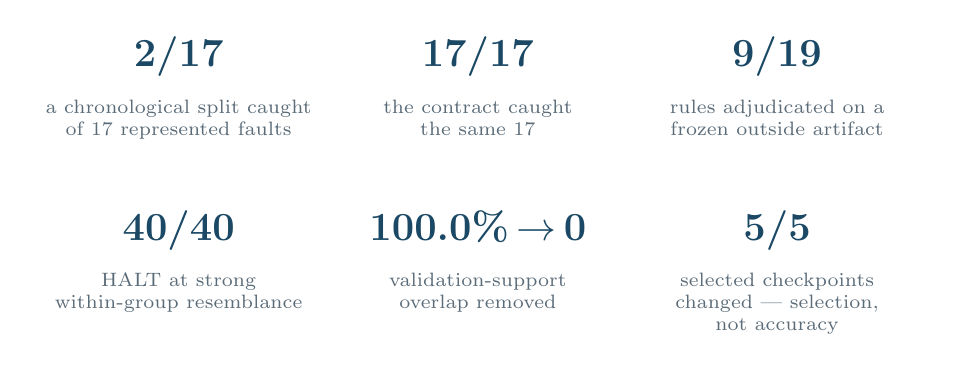
\begin{tikzpicture}[x=1mm,y=1mm]
    \foreach \xx/\yy/\num/\what in {%
        0/22/{\Nchrono/\Nfaults}/{a chronological split caught\\ of \Nfaults{} represented faults},
        38/22/{\Ncontract/\Nfaults}/{the contract caught\\ the same \Nfaults},
        76/22/{\Nextadjudicated/\Nextrules}/{rules adjudicated on a\\ frozen outside artifact},
        0/0/{\Nhaltshi/\Nseeds}/{HALT at strong\\ within-group resemblance},
        38/0/{\Nconsoverlap\%\,$\to$\,\Nconsoverlapcorr}/{validation-support\\ overlap removed},
        76/0/{\Nconschanged/\Nconsseeds}/{selected checkpoints\\ changed --- selection,\\ not accuracy}}%
      {\node[font=\Large\bfseries,text=oeaccent,anchor=north] at (\xx,\yy+9) {\num};
       \node[font=\scriptsize,text=oegrey,anchor=north,align=center,text width=36mm]
         at (\xx,\yy+1) {\what};}
  \end{tikzpicture}
  \punch{Not higher model accuracy --- an invalid experiment cannot support a deployment claim.}
\end{frame}

% 22 --------------------------------------------------------------- limits, as cards
\begin{frame}{What this does not establish}
  \centering
  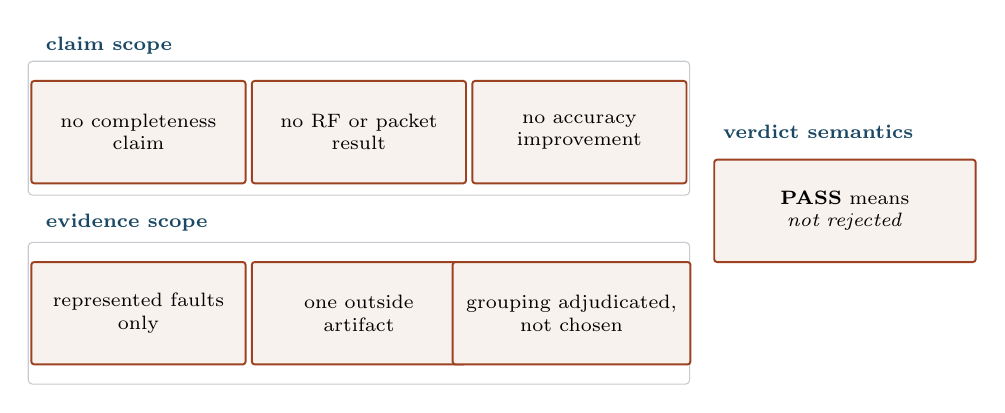
\begin{tikzpicture}[x=1mm,y=1mm]
    \draw[oegrey!35,rounded corners=1.5pt,line width=0.4pt] (-14,23) rectangle (70,6);
    \node[hdr,anchor=west] at (-13,25) {claim scope};
    \node[cardbad,text width=24mm,minimum height=13mm] at (0,14)  {no completeness\\claim};
    \node[cardbad,text width=24mm,minimum height=13mm] at (28,14) {no RF or packet\\result};
    \node[cardbad,text width=24mm,minimum height=13mm] at (56,14) {no accuracy\\improvement};
    \draw[oegrey!35,rounded corners=1.5pt,line width=0.4pt] (-14,0) rectangle (70,-18);
    \node[hdr,anchor=west] at (-13,2.5) {evidence scope};
    \node[cardbad,text width=24mm,minimum height=13mm] at (0,-9)  {represented faults\\only};
    \node[cardbad,text width=24mm,minimum height=13mm] at (28,-9) {one outside\\artifact};
    \node[cardbad,text width=27mm,minimum height=13mm] at (55,-9)
      {grouping adjudicated,\\ not chosen};
    \node[hdr,anchor=west] at (73,14) {verdict semantics};
    \node[cardbad,text width=30mm,minimum height=13mm,anchor=west] at (73,4)
      {\textbf{PASS} means\\ \emph{not rejected}};
  \end{tikzpicture}
  \punch{A validity method must apply its own evidence discipline to itself.}
\end{frame}

% 23 --------------------------------------------------------------- the three decisions
\begin{frame}{What I need from you}
  \centering
  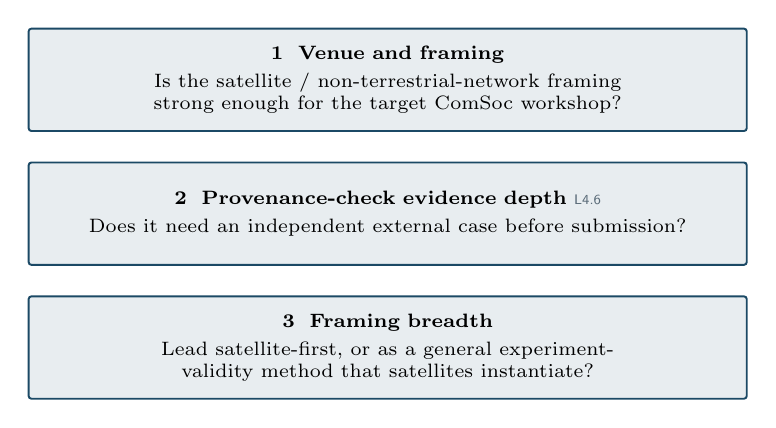
\begin{tikzpicture}[x=1mm,y=1mm]
    \node[card,text width=88mm,minimum height=13mm,fill=oeaccent!10,anchor=north] at (0,32)
      {\textbf{1\ \ Venue and framing}\\[0.25em]
       {\scriptsize Is the satellite / non-terrestrial-network framing strong enough for the
        target ComSoc workshop?}};
    \node[card,text width=88mm,minimum height=13mm,fill=oeaccent!10,anchor=north] at (0,15)
      {\textbf{2\ \ Provenance-check evidence depth}\ {\tiny\color{oegrey}\rulename{L4.6}}\\[0.25em]
       {\scriptsize Does it need an independent external case before submission?}};
    \node[card,text width=88mm,minimum height=13mm,fill=oeaccent!10,anchor=north] at (0,-2)
      {\textbf{3\ \ Framing breadth}\\[0.25em]
       {\scriptsize Lead satellite-first, or as a general experiment-validity method that
        satellites instantiate?}};
  \end{tikzpicture}
  \vspace{0.1em}

  {\scriptsize\color{oegrey} What is already settled: \Nclaimsites{} artifact-bound claim
   sites · \Nloc{}-line \texttt{numpy}-only toolkit · evidence frozen}
\end{frame}

% ================================================================= APPENDIX
\appendix

% A1 was a four-row layer summary that named only L4.6 and L4.7, so \Nrules{} rules were asserted
% and 2 were shown. Every rule is now accounted for individually -- an advisor asking "what are the
% other seventeen?" could not previously get an answer from the deck. Names are the registered
% identifiers in the frozen detector, not prose paraphrases.
\begin{frame}{A1 --- The complete \Nrules{}-rule map}
  \scriptsize
  \begin{columns}[T]
  \begin{column}{0.49\textwidth}
    \begin{tabular}{@{}ll@{}}
      \multicolumn{2}{@{}l}{\textbf{L1 --- availability \& membership} \hfill \emph{core}}\\
      \midrule
      L1.1 & feature availability\\
      L1.2 & availability clock\\
      L1.3 & label closure\\
      L1.4 & row membership\\
      L1.5 & comparison boundaries\\
      \addlinespace[0.5em]
      \multicolumn{2}{@{}l}{\textbf{L2 --- physical \& scheduling} \hfill \emph{support}}\\
      \midrule
      L2.1 & sampling geometry\\
      L2.2 & physical scale\hfill\textcolor{oewarn}{\tiny no red fixture}\\
      L2.3 & hidden state\hfill\textcolor{oewarn}{\tiny no red fixture}\\
      L2.4 & declared relation\\
    \end{tabular}
  \end{column}
  \begin{column}{0.49\textwidth}
    \begin{tabular}{@{}ll@{}}
      \multicolumn{2}{@{}l}{\textbf{L3 --- model-state causality} \hfill \emph{core}}\\
      \midrule
      L3.1 & state channels\\
      L3.2 & canary effectiveness\\
      L3.3 & negative control\\
      \addlinespace[0.5em]
      \multicolumn{2}{@{}l}{\textbf{L4 --- independence \& reproducibility} \hfill \emph{mixed}}\\
      \midrule
      L4.1 & chronology\\
      L4.2 & paired randomness\\
      L4.3 & repeated measures\\
      L4.4 & seed hygiene\\
      L4.5 & provenance hashes\hfill\textcolor{oewarn}{\tiny no red fixture}\\
      L4.6 & \textbf{provenance completeness}\\
      L4.7 & \textbf{statistical unit}\\
    \end{tabular}
  \end{column}
  \end{columns}
  \vspace{0.4em}

  {\scriptsize \Nred{} of \Nrules{} rules have a demonstrated red fixture; the \Nnored{} marked
  above do not. The two in bold are the paper's contribution; the other seventeen are the
  instantiation. \Nstatechannels{} probed state channels --- an operational enumeration, not a
  completeness claim. Detector source: \Nloc{} lines.}
\end{frame}

\begin{frame}{A2 --- The L4.7 permutation reference}
  \small
  Under the null the coarser grouping carries \emph{no} information, so unit values are
  exchangeable \textbf{across} the groups of $g$. The reference $\{\hat{\rho}^{*}\}$ comes from
  permuting unit values freely over \emph{all} units while the group memberships and sizes stay
  fixed --- so each draw keeps the observed group count and balance.
  \vspace{0.3em}

  {\footnotesize Permuting \emph{within} a group is a no-op: composition unchanged, every draw
   equal to $\hat{\rho}$.}
  \[ p = \frac{1 + \#\{\hat{\rho}^{*} \ge \hat{\rho}\}}{B+1}, \qquad B = \NpermB. \]
  {\footnotesize The $+1$ counts the observed statistic as one of its own reference draws, so the
   test is valid at any $B$ and the smallest reportable $p$ is $1/(\NpermB+1)$, not $0$. Every
   real-data HALT sits there.
   \vspace{0.25em}

   The numerator is unbiased, so the estimate can go negative and is reported truncated at zero.
   It uses the \emph{mean} group size, so on unbalanced data (\Natused{} units in \Natelsets{}
   groups) the estimate is a balanced-design approximation --- permutation referencing keeps the
   \emph{decision} size-valid either way. The one-sided bootstrap bounds $\Natlo$/$\Natupper$ are
   likewise \textbf{descriptive, not decision inputs}.}
\end{frame}

\begin{frame}{A3 --- Attainability versus power}
  \small
  \begin{tabular}{@{}lrrl@{}}
    \toprule
    design & assignments & smallest \emph{exact-reference} $p$ & reaches $\alpha=\Nalpha$?\\
    \midrule
    3 groups $\times$ 2 units & \Nassignthree & \Nminpthree & \textcolor{oewarn}{no}\\
    4 groups $\times$ 2 units & \Nassignfour  & \Nminpfour  & yes\\
    \bottomrule
  \end{tabular}
  \vspace{0.45em}

  Assignments for $k$ unlabelled groups of $m$ units: $(km)!/(m!^{k}k!)$ --- arithmetic about the
  \emph{design}, evaluated before any data is seen.
  \vspace{0.35em}

  \textbf{Two floors, two questions.} The column above is combinatorial: the smallest $p$
  attainable by the \emph{exact combinatorial} reference for that design. At \Nassignthree{} assignments it cannot reach
  $\alpha$ at all. The implemented rule is separate: it always draws $B=\NpermB$ random
  permutations, so the finest $p$ it \emph{reports} is $1/(\NpermB+1)$. A sampled reference could still emit $p\le\alpha$ by chance
  here; what prevents that is the precondition, not the sampling. It excludes only designs whose
  exact floor already exceeds $\alpha$, declining below \Nmingroups{} coarser groups or
  \Nminunits{} units --- exactly the \Nassignthree-assignment row.
\end{frame}

\begin{frame}{A4 --- Real-data denominator accounting}
  \small
  \begin{tabular}{@{}lr@{}}
    \toprule
    predicted-visible passes in the window (cohort) & \Npasses\\
    element-set records & \Nelsets\\
    objects & \Nobjects\\
    \midrule
    passes with no successor element set (no increment formable) & \Natdropped\\
    \textbf{passes entering the primary in-track analysis} & \textbf{\Natused}\\
    successor-paired element sets & \Natelsets\\
    \bottomrule
  \end{tabular}
  \vspace{0.5em}

  $\Npasses - \Natdropped = \Natused$. The two denominators are never merged: an increment needs
  \emph{two} consecutive records, so the \Natused{} passes are a \textbf{structurally selected
  subset} --- \emph{not} random missingness. No cohort-wide prevalence claim follows.
  \vspace{0.4em}

  A \textbf{third} denominator belongs here: the mean-elevation control runs over \Nelevunits{}
  units in \Nelevgroups{} element sets --- neither the cohort nor the along-track set. The
  one-sided bounds are a \Nbootdraws-draw bootstrap over coarser \emph{groups}, not the
  permutation reference.
\end{frame}

\begin{frame}{A5 --- Three clocks}
  \small
  \begin{tabular}{@{}lp{0.62\textwidth}@{}}
    \toprule
    element epoch & the state the element set describes\\
    CREATION\_DATE & when the record was created upstream\\
    retrieval time & when \emph{we} could actually obtain it\\
    \bottomrule
  \end{tabular}
  \vspace{0.5em}

  Availability reasoning needs the third, and only the second is published. So message-creation
  time is used as a \textbf{lower bound on retrievability}, never as exact retrieval time.
  \notclaim{that CREATION\_DATE is the exact moment the record became fetchable.}
\end{frame}

\begin{frame}{A6 --- The third-party L4.1 partition}
  \small
  Windows of \Nwindowspan{} samples slide by one sample, so adjacent windows share
  \Nboundarydropped{} of their \Nwindowspan{} samples. A shuffle-then-fraction split therefore
  places near-duplicates of validation windows into training.
  \vspace{0.4em}

  \begin{tabular}{@{}lrr@{}}
    \toprule
     & original & corrected\\
    \midrule
    overlap, \% of validation support & \Nconsoverlap\% & ---\\
    shared source timesteps & --- & \Nconsoverlapcorr\\
    boundary windows removed & 0 & \Nboundarydropped\\
    L4.1 verdict & HALT & PASS\\
    \bottomrule
  \end{tabular}
  \vspace{0.4em}

  The intervention changed \emph{only} the partition. Everything else --- architecture,
  hyper-parameters, seeds --- was held fixed, and the rerun is bit-identical.
\end{frame}

\begin{frame}{A7 --- Claim binding and reproducibility}
  \small
  \begin{itemize}\itemsep0.25em
    \item \Nclaimsites{} manuscript claim sites are bound to fields of the frozen summary
          artifact; the paper's gate refuses to build when one disagrees.
    \item Every number in this deck is generated from the same artifacts by
          \texttt{gen\_numbers.py} --- none is typed.
    \item The detector is byte-identical across the curated suite, the real-data application and
          the external study (same \texttt{contract\_layers\_sha256}).
    \item \Nenvs{} generator-family environments, \Nconds{} conditions each, deterministic across
          environments.
    \item \textbf{L4.6's precondition.} Its implication only holds if execution is
          \emph{deterministic given the declared} manifest --- otherwise a HALT is a disjunction
          (incomplete manifest \emph{or} nondeterminism). Established here, separately, by
          byte-identical rerun, which is why it is a reproducibility fact rather than part of the
          relational argument.
  \end{itemize}
\end{frame}

\begin{frame}{A8 --- Limitations matrix}
  \scriptsize
  \begin{tabular}{@{}p{0.30\textwidth}p{0.30\textwidth}p{0.32\textwidth}@{}}
    \toprule
    what is shown & what it licenses & what it does \emph{not} license\\
    \midrule
    \Ncontract/\Nfaults{} curated detection & regression reachability of represented faults &
      sensitivity to unseen faults\\[0.4em]
    $\hat{\rho}=\Naticc$, $p=\Natp$ & exchangeability rejected for this observable and hierarchy &
      the correct unit; a universal property\\[0.4em]
    external \Nextpass/\Nexthalt/\Nextindet & the frozen contract runs unmodified elsewhere &
      broad external generalisation\\[0.4em]
    checkpoint changed \Nconschanged/\Nconsseeds & the violation has a decision consequence &
      a downstream accuracy improvement\\
    \bottomrule
  \end{tabular}
\end{frame}

\begin{frame}{A9 --- Relationship to neighbouring work}
  \small
  \begin{tabular}{@{}lp{0.55\textwidth}@{}}
    \toprule
    metamorphic testing \srcref{Chen et al.\ 2018} & supplies the \emph{relation}; L4.6 supplies the \emph{target} ---
      declared provenance, where tracking systems record parameters without testing whether the
      declaration is behaviourally complete\\[0.5em]
    hermetic builds \srcref{Mokhov et al.\ 2018} & aim to \emph{prevent} undeclared inputs; L4.6 tests whether a declaration
      already in use is behaviourally complete\\[0.5em]
    pseudoreplication \srcref{Hurlbert 1984} & the statistical error L4.7 addresses; the contribution is turning its
      diagnosis into a calibrated, abstaining gate\\
    \bottomrule
  \end{tabular}
\end{frame}

\begin{frame}{A10 --- Historical motivation: the stopped Doppler-residual line}
  \begin{center}
  \fcolorbox{oewarn}{oewarn!8}{\begin{minipage}{0.95\textwidth}\centering
    \textbf{\textcolor{oewarn}{HISTORICAL MOTIVATION ONLY}}\\[0.15em]
    \textbf{\textcolor{oewarn}{NOT EVIDENCE FOR ORBIT-EVIDENCE}}
  \end{minipage}}
  \end{center}
  \vspace{0.5em}

  \small
  \begin{itemize}\itemsep0.32em
    \item An earlier line attempted a \textbf{learning-assisted satellite control problem}: a
          learned correction to a physical prediction, deployment gated on validation evidence.
    \item \textbf{Deployment-causality and falsifiability audits exposed problems a chronological
          split did not reveal} --- inputs unavailable at decision time, rows created by later
          information, state crossing the freeze, repeated measures treated as independent.
    \item Handled at first as individual bugs. \textbf{Generalising to what they shared} --- each
          needed a comparison outside one realised run --- produced relational validity.
  \end{itemize}

  {\footnotesize\textcolor{oewarn}{That line was stopped and its results are withdrawn. No
   quantitative result from it appears in this deck. Only the lineage is carried forward.}}
\end{frame}

% A11 --------------------------------------------------------------- the obvious repairs
% Every primitive this deck borrows, attributed. The deck argues that it invented none of its
% primitives, so naming them without references was the one integrity gap the scholarly pass had
% left open. Metadata is transcribed from paper/refs.bib -- nothing is cited here that the
% manuscript does not cite.
% A11 -- moved out of the main narrative by the visual-first redesign: it is an argument in
% prose, and the advisor reads figures. The point still matters for a reviewer, so it is kept
% whole here rather than deleted.
\begin{frame}{A11 --- Why the obvious repairs do not close the gap}
  \small
  \begin{tabular}{@{}p{0.30\textwidth}p{0.64\textwidth}@{}}
    \textcolor{oewarn}{\textbf{Stricter split}} &
      cannot see unpublished past-dated information, rows never created, hidden model state,
      or exchangeability\\[0.5em]
    \textcolor{oewarn}{\textbf{More single-run assertions}} &
      cannot falsify a relation whose counterexample needs a second execution\\[0.5em]
    \textcolor{oewarn}{\textbf{Richer provenance logging}} &
      cannot establish its own completeness --- a manifest may record every field its author
      recalled and still omit a behaviour-changing dependency\\[0.5em]
    \textcolor{oewarn}{\textbf{Aggregate first}} &
      choosing a level does not establish that the level is exchangeable\\
  \end{tabular}
  \msg{Each fails for the same reason: one realised run cannot supply the comparison.}
\end{frame}

% A12 --------------------------------------------------------------- references
\begin{frame}{A12 --- References for the borrowed primitives}
  \scriptsize
  \begin{enumerate}\setlength{\itemsep}{0.1em}\setlength{\parskip}{0pt}
    \item P.~E. Shrout and J.~L. Fleiss, ``Intraclass correlations: uses in assessing rater
      reliability,'' \emph{Psychological Bulletin}, 1979. \hfill{\scriptsize ICC(1)}
    \item A.~M. Winkler \emph{et al.}, ``Permutation inference for the general linear model,''
      \emph{NeuroImage}, 2014. \hfill{\scriptsize permutation reference}
    \item E.~B. Wilson, ``Probable inference, the law of succession, and statistical inference,''
      \emph{J.~Amer. Statist. Assoc.}, 1927. \hfill{\scriptsize binomial interval}
    \item S.~H. Hurlbert, ``Pseudoreplication and the design of ecological field experiments,''
      \emph{Ecological Monographs}, 1984. \hfill{\scriptsize the unit error L4.7 targets}
    \item T.~Y. Chen \emph{et al.}, ``Metamorphic testing: a review of challenges and
      opportunities,'' \emph{ACM Computing Surveys}, 2018. \hfill{\scriptsize relations over runs}
    \item A.~Mokhov \emph{et al.}, ``Build systems \`a la carte,'' \emph{Proc. ACM on Programming
      Languages}, 2018. \hfill{\scriptsize hermetic dependency closure}
    \item C.~Bergmeir and J.~M. Ben\'{\i}tez, ``On the use of cross-validation for time series
      predictor evaluation,'' \emph{Information Sciences}, 2012.
      \hfill{\scriptsize when ordered splitting is valid}
    \item K.~Hundman \emph{et al.}, ``Detecting spacecraft anomalies using LSTMs and nonparametric
      dynamic thresholding,'' \emph{Proc. KDD}, 2018. \hfill{\scriptsize the frozen third-party artifact}
  \end{enumerate}
  {\scriptsize\itshape\color{black!70}The primitives are all prior art. The \textbf{conversion} is the contribution.}
\end{frame}

\end{document}
